\chapter{Supplement -- Performance Modeling}
\label{App_A:Perf_Model}
\chaptertoc

\section{Related Performance Models for Work Stealing}
\label{App_A:related_models_workstealing}

In this appendix, we summarize the previous performance models for work stealing. The first model is work stealing without communication latency \cite{tchiboukdjian2010tighter} \cite{tchiboukdjian2013decentralized}. The second model is also work stealing but with latency proposed by \cite{gast2021analysis} in 2021.\\

The main purpose of performance modeling is to show an upper bound of balancing efficiency, such as the number of tasks that can be migrated. Extended from the original work \cite{Blumofe1999OriginWS}, Tchiboukdjian et al. have proposed a good model for work stealing without latency since 2010 \cite{tchiboukdjian2010tighter} \cite{tchiboukdjian2013decentralized}.\\

\begin{figure}[t]
  \centering
  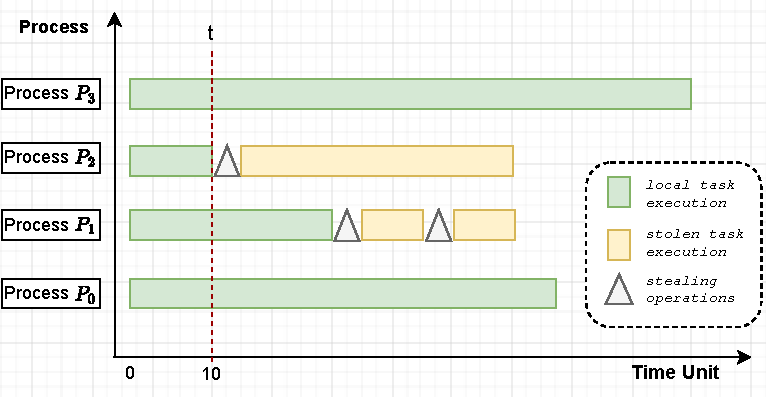
\includegraphics[scale=0.8]{./pictures/perf_analysis_model/perf_analysis_related_model_without_latency.pdf}
	\caption{An illustration of work stealing without latency.}
	\label{fig:perfmodel_relatedmodelwithoutlatency}
\end{figure}

To summarize the related performance models, we illustrate an example of work stealing behaviors in Figure \ref{fig:perfmodel_relatedmodelwithoutlatency}. The x-axis shows the progress over execution time along with four processes indexed from $P_{0}$ to $P_{3}$. The triangles represent stealing operations at a time. This is an ideal case for load balancing when the overhead of sending and receiving tasks is almost instantaneous. This example is known as task execution in shared memory systems. As we know, in work stealing, idle processes try to steal tasks from busy processes. Communication is assumed to be very fast in sending and receiving tasks.\\

To demystify the related models, we summarize the terminologies and notations that their authors used in Table \ref{tab:mapped_notation_table}; comparing to the notations used in this thesis. We try to address them separately to avoid a conflict. For example,  this thesis formulates a given distribution of $T$ on $P$ processes, where each holds a subset of $T_{i}$ tasks. In the related performance models, the authors use $w_{i}$ to indicate the number of tasks in process $P_{i}$  \cite{tchiboukdjian2013decentralized}. We try to make this consistent by using $T_{i}$ as the number of tasks in process $P_{i}$. In the following sections, there might be some additional notations about the queue information, e.g., $Q_{i}$ represents the queue status denoted by the values of the number of tasks. Mapping them to the time progress, this may have the field of time $(t)$. For instance, $T_{i}(t)$ means the number of tasks in process $P_{i}$ at time $t$, or $T(t)$ without $i$ means the total number of tasks (for all processes) at time $t$. The text might re-mention these notations in some specific paragraphs when we want to show further explanation.\\

\begin{table}[t]
\centering
\begin{tabular}{|l|p{2cm}|p{5cm}|p{4.5cm}|}
\hline
\textbf{No.} & \textbf{Notations} & \textbf{Description} & \textbf{Note}        \\ \hline
1  & $T$          & the number of tasks indexed $\left \{0,...,(T-1) \right \}$ & In the related works, people used $W$ instead of $T$   \\ \hline
2  & $P$					& the number of processes, $\left \{0,...,(P-1) \right \}$    & The related works used $m$ identical processors instead of $P$ \\ \hline
3  & $T_{i}$			& the set of assigned tasks in process $P_{i}$                & The related works used $w_{i}$ instead of $T_{i}$              \\ \hline
4  & $L_{i}$			& the total load of process $P_{i}$                           &                                             \\ \hline
5  & $w_{i}$			& the wallclock execution time of a task, i.e., task $i$      &                                             \\ \hline
6  & $W_{i}$ 			& the wallclock execution time of process $P_{i}$             &                                             \\ \hline
7  & $S_{P_{i}}$	& processing speed (performance model) of process $P_{i}$     &                                             \\ \hline
8  & $Slow_{i}$		& slowdown coefficient of process $P_{i}$ at runtime          &                                             \\ \hline
9  & $W_{par}$		& the total wallclock execution time (makespan)               & Also called completion time ($C$)           \\ \hline
10 & $R_{imb}$		& imbalance ratio                                             &                                             \\ \hline
11 & $\lambda$		& communication or network latency                            &                                             \\ \hline
12 & $d$					& delay or transmission time                                  &                                             \\ \hline
13 & $B$					& network bandwidth                                           &                                             \\ \hline
14 & $O_{ij}(t)$	& the number of offloaded tasks from process $P_{i}$ to $P_{j}$  & The authors in \cite{tchiboukdjian2010tighter} used $R(t)$ as the number of task requests in global after time $t$ \\ \hline
\end{tabular}
\caption{Used notations in the thesis comparing to the notations from related works.}
\label{tab:mapped_notation_table}
\end{table}


\noindent \textbf{A. A Tight Analysis of Work Stealing \cite{tchiboukdjian2010tighter,tchiboukdjian2013decentralized}}\\

In \cite{tchiboukdjian2013decentralized}, Tchiboukdjian et al. considered a parallel platform with $P$ processes. At time $t$, $T_{i}(t)$ represents the amount of works\footnote{Works are considered as tasks. Therefore, they might be used interchangeably.} on process $P_{i}$. Compared to $t=0$, $T_{i}(t)$ will be decreased by time progress. For example, at $t=0$ the workload is distributed on each process, $T_{i}(t_{0}) = 100$ means having 100 tasks before running. Then, at $t=10$ we assume 10 tasks have been done on process $P_{i}$, and $T_{i}(t_{10})$ would be $90$ as the remaining tasks. Taking Figure \ref{fig:perfmodel_relatedmodelwithoutlatency} as an example, at $t=10$ process $P_{3}$ has done 10 tasks, and its queue remains 90 tasks, $T_{0}(t_{10}) = 90$. In contrast, process $P_{2}$ is faster and it has done all tasks at $t=10$, therefore, $T_{2}(t_{10}) = 0$. In general, the execution behavior can be simplified as follows, where a processor also refers to a process.

\begin{itemize}
	\item when $T_{i}(t) > 0$, Processor $i$ is active and execute tasks, $T_{i}(t+1) \leq T_{i}(t)$.
	\item when $T_{i}(t) = 0$, Processor $i$ is idle and intends to steal tasks from a random processor $j$.
\end{itemize}

If work stealing is applied, some tasks are migrated, then $T_{i}(t)$ will increase or decrease, depending on how many steal requests and tasks are performed at a time. Tchiboukdjian et al. \cite{tchiboukdjian2010tighter} \cite{tchiboukdjian2013decentralized} assumed that between time $t$ and $t+1$, there are $P - \alpha(t)$ steal requests, $P$ denotes the total number of processes and $\alpha(t)$ denotes the number of active processes, $\alpha(t) \in [0, m]$. When $\alpha(t)=0$, it means all queues are empty as well as the execution is complete. Corresponding to the sucess steal requests, process $P_{j}$ transfers an amount of works to process $P_{i}$ and $T_{i}(t+1) + T_{j}(t+1) \leq T_{j}(t)$. Similarly, when $\alpha(t)=0$, the execution terminates if $\forall i \in P, T_{i}(t) = 0$. At time $t$, the total number of tasks of all processes is denoted by $T(t) = \sum_{i=1}^{P}T_{i}(t)$. After that, process $P_{2}$ steals some tasks from the others to help balance the load. The triangle shows stealing operations, and there is obviously stealing overhead in practice. However, we show this model with an assumption about no latency, in which the use cases might be considered in shared memory.\\

In the baseline without work-stealing, the total execution time depends on the process with a maximum load, $C_{max} = max_{i \in P} T_i(t_0)$. When we apply work stealing, $C_{max}$ can be reduced. Following that, the main question is:
\begin{shaded}
	\noindent What is the upper bound of makespan when work stealing is applied?
\end{shaded}

The work \cite{tchiboukdjian2010tighter} has proposed a potential function $\Phi (t)$ to model the performance of work stealing by studying the potential decrease. Assuming that tasks are unit independent, $\Phi (t)$ is defined by
\begin{equation} \label{eq:phi_defi}
	\Phi(t) = \sum_{i=1}^{P} (T_{i}(t) - \frac{T(t)}{P})^{2} = \sum_{i=1}^{P} T_{i}(t)^{2} - \frac{T(t)^2}{P}
\end{equation}
where, the potential represents the load imbalance of execution. For example, as expected at time $t$ the average load among $P$ processes is $\frac{T(t)}{P}$. If we sum the difference at time $t$ between the load value of each process and the average load value, the result shows the load difference level. \\

Therefore, the decrease of $\Phi (t)$ depends on the number of steal requests and execution scenario. The above has mentioned an estimated formula for the number of steal requests ($P - \alpha(t)$). $\alpha(t)$ is a complicated random process that chooses the number of active processors at each step. Such an expectation in work-stealing, the more work requests it creates, the more the potential will decrease. The performance analysis model is performed in three steps:
\begin{enumerate}
	\item Define $\Phi (t)$.
	\item Compute the expected decrease of $\Phi (t)$ between time step $t$ and $t+1$, $\Delta \Phi (t) \overset{def}{=} \Phi (t) - \Phi (t+1)$. However, at a specific time $t$, how can we estimate the decrease? The authors define another term, named $\delta_{i}^{k}(t)$, to compute the expected decrease,
	\begin{equation} \label{eq:expect_decrease}
		\sum_{i=1}^{P} \sum_{k=0}^{P-1} E [\delta_{i}^{k}|i\ \textrm{receives}\ k\ \textrm{requests}]P\left \{ i\ \textrm{receives}\ k\ \textrm{requests} \right \}
	\end{equation}
	
 , where the first sum goes through all $P$ processes and the second sum goes from $0$ to $(P-2)$ as the maximum requests a process can get at a time. $E[X|Y]$ denotes the expectation of $X$ knowing $Y$. Applying this to the example in Figure \ref{fig:perfmodel_relatedmodelwithlatency} we have
	
	\begin{equation}
		E[\Delta \Phi (t)] = \sum_{i=0}^{3} \sum_{k=0}^{3} E [\delta_{i}^{k}|i\ \textrm{receives}\ k\ \textrm{requests}]P\left \{ i\ \textrm{receives}\ k \textrm{requests} \right \}
	\end{equation}

	Following that, the authors showed that there exists a function called $h(\alpha) \in (0;1]$ such that $E[\Delta \Phi (t)|\Phi (t) = \Phi,\alpha(t) = \alpha] \geq h(\alpha) \Phi$.
	
	\item The work \cite{tchiboukdjian2010tighter} obtained a bound on the expected number of steal requests $E[R]$ ($R$ is the number of steal requests), and the expected makespan $E[C_{max}]$ can be further obtained from $E[R]$.
\end{enumerate}

Tchiboukdjian et al. \cite{tchiboukdjian2010tighter} concluded that the expected number of steal requests $R$ until $\Phi(t) \leq 1$ is bounded by $E[R] \leq \lambda \cdot P \cdot log_{2} \Phi(0)$, where $\lambda$ in this case is $max_{1 \leq \alpha \leq P-1} \frac{P-\alpha}{-P \cdot log_{2}(1-h(\alpha))}$ and $\Phi(0)$ is the potential at $t=0$. At the end, the expected value of $C_{max}$ will be bounded by 
\begin{equation}
	E[C_{max}] \leq \frac{T}{P} + \frac{2}{1-\log_{2}(1+\frac{1}{\epsilon})} \log_{2}W + 1
\end{equation}

Before \cite{tchiboukdjian2010tighter,tchiboukdjian2013decentralized}, some previous works also attempted to find an upper bound. One of the original studies from Blumofe and Leiserson \cite{Blumofe1999OriginWS} showed that the efficiency of work stealing is bounded by $E(C_{max}) \leq \frac{T}{P} + O(D)$, where $D$ is the length of the critical path in the case of dependent tasks (a task graph). The analysis is further improved by \cite{arora2001thread} using potential functions. The authors used an amortization argument based on a potential function that decreases the work stealing algorithm processes. The idea is to divide the execution into phases and show that the potential decreases by at least a constant fraction with a constant probability. For the case of varying the speed of $P$ processors or heterogeneous processors, Bender and Rabin \cite{bender2002online} provided a new analysis of an old scheduling algorithm called \textit{maximum utilization scheduler}. The authors showed a given context for $P$ processors with speed $\pi_{i}$ steps/time. These studies are constrained in the context of only one source of tasks, which could not easily model the basic case of independent tasks, and communication overhead is not explicitly counted.\\

\noindent \textbf{B. A Tighter Analysis of Work Stealing with Latency \cite{gast2021analysis}} \\

For a performance model with communication latency, Nicolas Gast et al. \cite{gast2021analysis} proposed a new analysis model on how communication latency impacts stealing operations in terms of task-parallel applications. The model has been created for distributed memory clusters with $P$ identical processors. The latency value is denoted by $\lambda$. This research is inherited from the previous work \cite{tchiboukdjian2013decentralized} and aimed at an upper bound for an expected makespan.\\

From the previous study \cite{tchiboukdjian2013decentralized}, the authors also make a consistent assumption about work stealing algorithms as follows:
\begin{itemize}
	\item The total number of processes is defined as $P$ identical processors.
	\item $T_{i}(t)$ denotes the amount of tasks on processor $i$ at time $t$, while the total tasks at time $t$ is $T(t) = \sum_{i=1}^{P}T_{i}(t)$. 
	\item A task corresponds to a unit of execution time.
	\item Regarding communication latency, all operations take the same $\lambda \in N$ time unit.
	\item Single Task Transfer: a processor can send some tasks to at most one processor at a time.
	\item Steal Threshold: if the victim has less than $\lambda$ task units to execute, the stealing request will be failed.
	\item Task to be stolen: the victim sends to the thief half of its tasks at a time. For example, the total tasks of process $P_{i}$ at time $t$ is $T_{i}(t) = \frac{T_{i}(t-1) - 1}{2}$.
\end{itemize}

\begin{figure}[t]
  \centering
  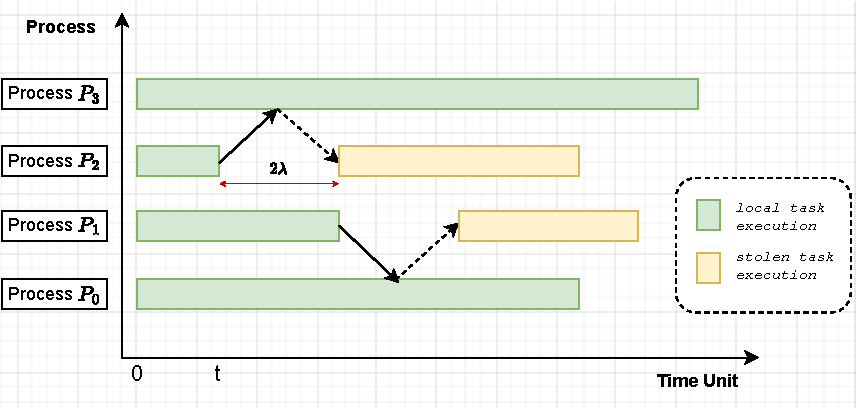
\includegraphics[scale=0.8]{./pictures/perf_analysis_model/perf_analysis_related_model_with_latency.pdf}
	\caption{An illustration of work-stealing with latency effect.}
	\label{fig:perfmodel_relatedmodelwithlatency}
\end{figure}

Figure \ref{fig:perfmodel_relatedmodelwithlatency} demonstrates a scenario of work stealing with latency. The x-axis represents the time progress of execution with four involved processes. Process $P_{2}$ is assumed idle and sends a steal request to process $P_{3}$. Since process $P_{3}$ accepts, task is sent from $P_{3}$ to $P_{2}$. Nicolas Gast et al. \cite{gast2021analysis} name $\lambda$ as the latency, and one stealing action takes a round-trip time $2\lambda$. This occurs similarly between process $P_{1}$ and $P_{0}$.\\

As the round-trip time of $2\lambda$ and the total amount of tasks $T$ on $P$ processes, Nicolas Gast et al. introduce a straightforward bound of makespan as \ref{eq:straight_cmax}.
\begin{equation} \label{eq:straight_cmax}
\begin{split}
	P \cdot & C_{max} \leq T + 2\lambda \cdot \#{\textrm{task requests}} \\
	\Leftrightarrow \ & C_{max} \leq \frac{T}{P} + 2\lambda \cdot \frac{\#{\textrm{task requests}}}{P}
\end{split}
\end{equation}

However, to be closer to an optimal bound, this work \cite{gast2021analysis} approached a potential function bounding on the number of work stealing requests\footnote{Work-stealing requests mean the number of requests for stealing tasks. Therefore, it is also called $\#{\textrm{task requests}}$ shown in Equation \ref{eq:straight_cmax} or steal requests}. The authors reconsidered the time division as periods of duration $\lambda$ to analyze the impact of latency. To not abuse notations, we use $T_{i}(k)$ and $s_{i}(k)$ to denote the current number of tasks and the number of stolen tasks from process $P_{i}$ at time $k$; then the quantities will be $T_{i}(k\lambda)$, $s_{i}(k\lambda)$. In the interval $(\lambda (k-1), \lambda k]$, the total number of incoming work stealing requests is defined by $r(k) = \sum_{i=1}^{\lambda} R((k-1)\lambda + i)$, where $0 \leq r(k) \geq P$. The probability, that a process receives $\geq 1$ requests in the interval $(\lambda (k-1), \lambda k]$, is $q(r(k))$.\\

Nicolas Gast et al. \cite{gast2021analysis} showed the analysis of the potential decrease, which is defined in Equation \ref{eq:potfunc_latency} at time-step $k\lambda$.
\begin{equation} \label{eq:potfunc_latency}
\begin{split}
	\Phi(k) = 1 + \frac{1}{\lambda^2} \sum_{i=1}^{P} (T_{i}(k)^2 + 2s_{i}(k)^2)
\end{split}
\end{equation}

where, $\Phi(k)$ gets through all processes $\in P$, $T_{i}(k)$ and $s_{i}(k)$ represents the number of remaining tasks as well as the number of stolen tasks in process $P_{i}$ at time $k$. Let $\Phi(0)$ be the potential at time $t_{0}$ and $\tau$ be the first time step at which the potential reaches $1$. Then, Nicolas Gast et al. proved that the number of incoming steal requests until $\tau$, $R = \sum_{k=0}^{\tau = 1} r(k)$ satisfies:
\begin{equation} \label{eq:exp_prob_R_latency}
\begin{split}
	& E[R] \leq P \gamma \log_{2} \Phi(0) \\
	& \mathbb{P}[R \leq P \gamma (\log_{2} \Phi(0) + x)] \leq 2^{-x}
\end{split}
\end{equation}

Where, $E[R]$ is the expected number of total incoming steal requests and $\mathbb{P}$ indicates the probability when $R \leq P \gamma (\log_{2} \Phi(0) + x)$, and $\gamma$ is a constant such that $\gamma < 4.03$. Applying to $C_{max}$, the study concluded as Equation \ref{eq:exp_prob_Cmax_latency} shows.

\begin{equation} \label{eq:exp_prob_Cmax_latency}
\begin{split}
	& E[C_{max}] \leq \frac{T}{P} + 4\lambda\gamma\log_{2} \frac{P}{\lambda} + 2\lambda\gamma \\
	& \mathbb{P}[C_{max} \geq \frac{T}{P} + 4\lambda\gamma\log_{2} \frac{P}{\lambda} + x] \leq 2^{\frac{-x}{2\lambda\gamma}}
\end{split}
\end{equation}


\paragraph{Further discussion:}
The related models above are relevant in terms of work stealing with or without latency. However, latency $\lambda$ is considered as a constant, and the number of steal requests must contribute relatively, such as task execution time. These constraints might be limited by the cases that task data sizes differ and transmission time considerably impacts the efficiency of stealing operations in practice. In contrast, this thesis analyzes the performance in a different direction. We introduce a model associated with transmission time (delay time) in HPC. The delay happens when tasks are migrated in distributed memory. First, the delay values depend on the size of task data in movement and the current status of interconnection, e.g., latency and bandwidth. Second, we show that this challenge can negatively impact the decision time of taking stealing or balancing actions. This is why it delays dynamic load balancing in distributed memory.

% We will discuss a proposed model with delay time when tasks are migrated.

%\section{Reactive load balancing simulation}
%\label{App_A:reactlb_sim}
